\documentclass[12pt,a4paper]{article}
\usepackage[utf8]{inputenc}
\usepackage[french]{babel}
\usepackage[T1]{fontenc}
\usepackage{amsmath}
\usepackage{amsfonts}
\usepackage{amssymb}
\usepackage{graphicx}
\author{KONDI Abdoul malik \\ NGANDEU NDJEUKAM Alhasan}
\title{Étude prévisionnel du projet de gestion d'une librairie}
\begin{document}
\maketitle
\tableofcontents
\newpage

\section{Planning}

<<<<<<< HEAD
=======
\begin{center}
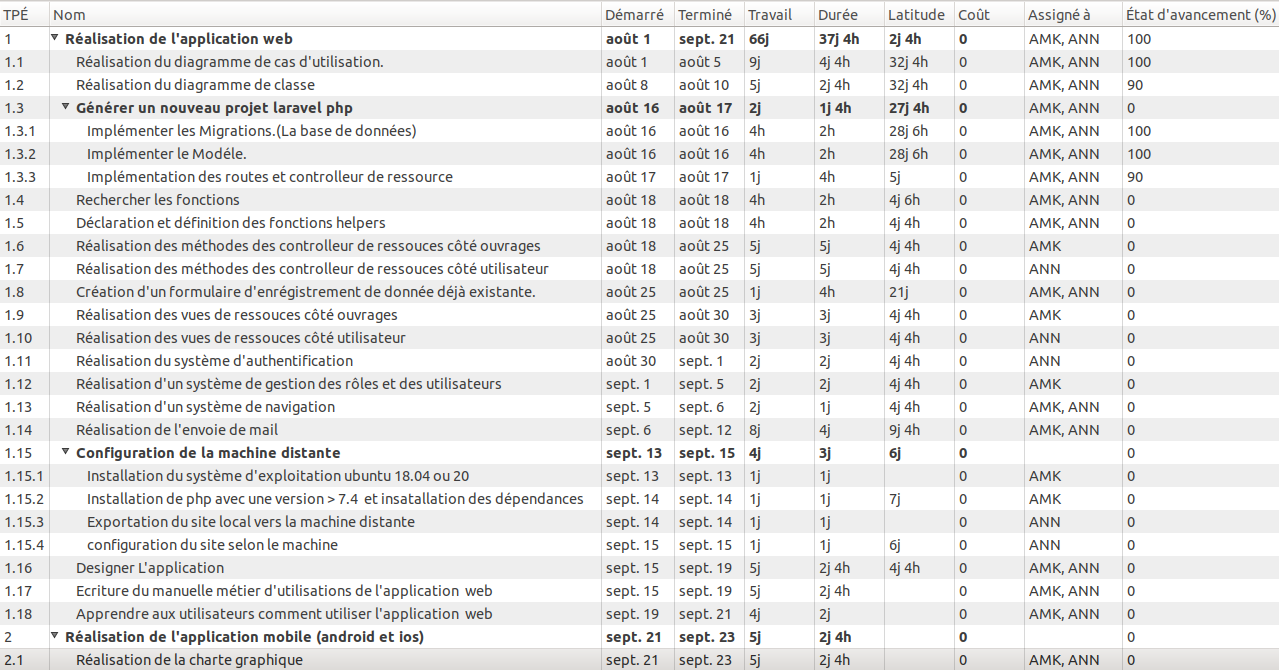
\includegraphics[width=16cm]{images/taches.png}
\end{center}
>>>>>>> f36fbfa2ce94707c4eccb761d033aaf9c48a0cec

\newpage

\section{Résumé récapitulatif du planning:}
\begin{center}
\begin{tabular}{|c|c|p{6cm}|p{4cm}|}
\hline 
Début & Fin & Tâche à accomplir & Besoin \\ 
\hline 
\textbf{01/08/2022} & \textbf{13/08/2022} & Réalisation du modèle & maître de stage\\ 
\hline 
\textbf{15/08/2022} & \textbf{17/08/2022} & Initialisation du projet et création de la base de données & maître de stage \\ 
\hline
\textbf{18/08/2022} & \textbf{25/08/2022} & \begin{itemize}
\item[•] Pouvoir ajouter de nouveaux livres en saisissant l’ISBN
\item[•] Indexer et classer les livres dans différentes catégories/rubriques
\item[•] Permettre au gérant de la médiathèque de gérer des ouvrage physiques pour les abonné
\end{itemize} & Liste des livres à la Bibliothèque \\ 
\hline 
\textbf{25/08/2022} & \textbf{06/09/2022} & \begin{itemize}
\item[•] Ranger les livres sous forme de tableau
\item[•] Rendre accessibles les livre simultanément par plusieurs centaines d’utilisateurs
\item[•] Faire la recherche d’un ouvrage à partir de certains critères (auteur, titre, ISBN...)
\item[•] Afficher la liste des ouvrages disponibles classés par catégorie
\item[•] Possibilité pour les utilisateurs de consulter en ligne plus de 2000 livres
\end{itemize} & 
\begin{itemize}
\item[•] Livres numérique
\item[•] Documents audio visuel
\end{itemize} \\
\hline 
\end{tabular} 
\end{center}

\newpage

\begin{center}
\begin{tabular}{|c|c|p{6cm}|p{4.5cm}|}
\hline 
 &  & \begin{itemize}
\item[•] Décrire chaque document (PDF) avec ses propriétés titre, auteurs et si possible donner une
\item[•] Table des matières qui lui est associée
\item[•] Donner la possibilité aux utilisateurs de la bibliothèque numérique de télécharger des livres au
format PDF
\end{itemize} & \\
\hline 
\textbf{30/08/2022} & \textbf{02/09/2022} & Configuration de la machine distante et déploiement & 
\begin{itemize}
\item[•] Machine distante pour l'hébergement.
\item[•] Machine physique pour le personnel de la médiathèque.
\end{itemize} \\
\hline 
\textbf{05/09/2022} & \textbf{07/09/2022} & Designer l'application & - \\
\hline 
\textbf{08/09/2022} & \textbf{12/09/2022} & Écriture du manuel d'utilisation & - \\ 
\hline
\textbf{12/09/2022} & \textbf{14/09/2022} & Apprendre l'utilisation de l'application aux utilisateurs & personnels\\ 
\hline  
\textbf{14/09/2022} & \textbf{16/09/2022} & Réalisation de l'application mobile(android \& ios) & -\\ 
\hline 
\end{tabular} 
\end{center}



\end{document}




